\documentclass{standalone}
\usepackage{tikz}
\usetikzlibrary{shapes.geometric}
\begin{document}
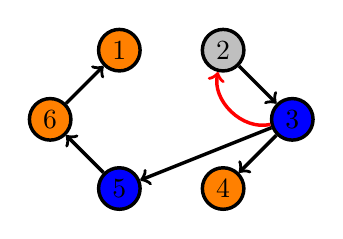
\begin{tikzpicture}
[every node/.style={inner sep=0pt}]
\node (1) [circle, minimum size=15.0pt, fill=orange, line width=1.25pt, draw=black] at (50.0pt, -25.0pt) {\textcolor{black}{1}};
\node (2) [circle, minimum size=15.0pt, fill=lightgray, line width=1.25pt, draw=black] at (87.5pt, -25.0pt) {\textcolor{black}{2}};
\node (3) [circle, minimum size=15.0pt, fill=blue, line width=1.25pt, draw=black] at (112.5pt, -50.0pt) {\textcolor{black}{3}};
\node (4) [circle, minimum size=15.0pt, fill=orange, line width=1.25pt, draw=black] at (87.5pt, -75.0pt) {\textcolor{black}{4}};
\node (5) [circle, minimum size=15.0pt, fill=blue, line width=1.25pt, draw=black] at (50.0pt, -75.0pt) {\textcolor{black}{5}};
\node (6) [circle, minimum size=15.0pt, fill=orange, line width=1.25pt, draw=black] at (25.0pt, -50.0pt) {\textcolor{black}{6}};
\draw [line width=1.25, ->, color=black] (6) to  (1);
\draw [line width=1.25, ->, color=black] (2) to  (3);
\draw [line width=1.25, ->, color=black] (3) to  (4);
\draw [line width=1.25, ->, color=black] (5) to  (6);
\draw [line width=1.25, ->, color=black] (3) to  (5);
\draw [line width=1.25, ->, color=red] (3) to  [in=257, out=193] (2);
\end{tikzpicture}

\end{document}
